% APLAS 2021: Regular research papers should not exceed 18 pages in
% the Springer LNCS format(LaTeX template), including bibliography and
% figures.
% Lightweight double-blind: Author names and institutions must be
% omitted and References to the authors’ own related work should be in
% the third person 
%
\documentclass[runningheads]{llncs}
\pdfoutput=1
%\usepackage[english]{babel}
\usepackage[utf8]{inputenc}
\usepackage{amsmath}
\usepackage{amssymb}
%\usepackage{graphicx}
%\usepackage[colorinlistoftodos]{todonotes}
\usepackage{mathpartir}
\usepackage{graphicx}
%\usepackage{fixme}
\usepackage{xcolor}
\usepackage{hyperref}
\usepackage{listings}

%%% structure
\newcommand{\Angle}[1]{\langle#1\rangle}

%% values
\newcommand{\NEG}{\neg}
\newcommand{\CNF}{\wedge}
\newcommand{\DNF}{\vee}
\newcommand{\TRUE}{\text{True}}
\newcommand{\FALSE}{\text{False}}
\newcommand{\EMPTYSTRING}{\text{$""$}}
\newcommand{\STACKCONCAT}{\text{$::$}}
\newcommand{\ZERO}{\text{0}}
\newcommand{\ONE}{\text{1}}
\newcommand{\VAMOUNT}{\text{amount}}
\newcommand{\VCONTRACT}{\text{contract}}

%% contract constants
\newcommand{\CAMOUNT}{\text{amount}}
\newcommand{\CBALANCE}{\text{balance}}
\newcommand{\CSENDER}{\text{sender}}
\newcommand{\CSOURCE}{\text{source}}
\newcommand{\CNOW}{\text{now}}
\newcommand{\CLEVEL}{\text{level}}
\newcommand{\CCHAINID}{\text{chain-id}}
\newcommand{\CSELF}{\text{self}}
\newcommand{\CSELFADDRESS}{\text{self-address}}
\newcommand{\CTOTALVOTINGPOWER}{\text{total-voting-power}}
\newcommand{\CVOTINGPOWER}{\text{voting-power}}

%% contract instructions
\newcommand{\AMOUNT}{\text{AMOUNT}}
\newcommand{\BALANCE}{\text{BALANCE}}
\newcommand{\SENDER}{\text{SENDER}}
\newcommand{\SOURCE}{\text{SOURCE}}
\newcommand{\NOW}{\text{NOW}}
\newcommand{\LEVEL}{\text{LEVEL}}
\newcommand{\CHAINID}{\text{CHAIN-ID}}
\newcommand{\SELF}{\text{SELF}}
\newcommand{\SELFADDRESS}{\text{SELF-ADDRESS}}
\newcommand{\TOTALVOTINGPOWER}{\text{TOTAL-VOTING-POWER}}
\newcommand{\VOTINGPOWER}{\text{VOTING-POWER}}
\newcommand{\MinusBalanceAmount}{\text{BALANCE-AMOUNT}}
%% auction contract
\newcommand{\AuctionOwner}{\text{auction-owner}}
\newcommand{\AuctionBidder}{\text{auction-bidder}}
\newcommand{\AuctionClose}{\text{auction-close}}
\newcommand{\AuctionOpen}{\text{auction-open}}
\newcommand{\AuctionBid}{\text{auction-bid}}

%% system definition
\newcommand{\VAL}{\textbf{v}}
\newcommand{\VAR}{\textbf{x}}
\newcommand{\VARIABLE}{\text{$Var$}}
\newcommand{\CONSTANT}{\text{$Const$}}
\newcommand{\TERM}{\text{$T$}}
\newcommand{\VariableX}{\text{$x$}}
\newcommand{\VariableV}{\text{$v$}}
\newcommand{\VariableK}{\text{$k$}}
\newcommand{\VariableA}{\text{$a$}}
\newcommand{\VariableB}{\text{$b$}}
\newcommand{\ELT}{\text{$Elt$}}
\newcommand{\A}{\text{$A$}}
\newcommand{\B}{\text{$B$}}
\newcommand{\N}{\text{$n$}}
\newcommand{\K}{\text{$k$}}
\newcommand{\V}{\text{$v$}}
\newcommand{\M}{\text{$m$}}
\newcommand{\VariableOne}{\text{$x_1$}}
\newcommand{\VariableTwo}{\text{$x_2$}}
\newcommand{\VariableN}{\text{$x_n$}}
\newcommand{\Constant}{\text{$c$}}
\newcommand{\ConstantOne}{\text{$c_1$}}
\newcommand{\ConstantTwo}{\text{$c_2$}}
\newcommand{\ConstantN}{\text{$c_n$}}
\newcommand{\LIST}{\text{$l$}}
\newcommand{\EMPTYLIST}{\text{$\{\}$}}
\newcommand{\TLIST}{\text{$l'$}}
\newcommand{\HEAD}{\text{$hd$}}
\newcommand{\TAIL}{\text{$tl$}}
\newcommand{\STAIL}{\text{$< tl >$}}
\newcommand{\Term}{\text{$t$}}
\newcommand{\TermOne}{\text{$t_1$}}
\newcommand{\TermTwo}{\text{$t_2$}}
\newcommand{\TermN}{\text{$t_n$}}
\newcommand{\TermB}{\text{$t_b$}}
\newcommand{\STACK}{\text{$S$}}
\newcommand{\EMPTYSTACK}{\text{[ ]}}
\newcommand{\STACKONE}{\text{$S$}}
\newcommand{\STACKTWO}{\text{$S$}}
\newcommand{\STACKN}{\text{$S$}}
\newcommand{\Stack}{\text{$s$}}
\newcommand{\StackOne}{\text{$s_1$}}
\newcommand{\StackTwo}{\text{$s_2$}}
\newcommand{\StackN}{\text{$s_n$}}
\newcommand{\TSTACK}{\text{$S'$}}
\newcommand{\TStack}{\text{$s'$}}
\newcommand{\STATE}{\text{$ST$}}
\newcommand{\STATEONE}{\text{$ST_1$}}
\newcommand{\STATETWO}{\text{$ST_2$}}
\newcommand{\STATEN}{\text{$ST_n$}}
\newcommand{\SYSTEM}{\text{$SE$}}
\newcommand{\INSTRUCTION}{\text{$I$}}
\newcommand{\TINSTRUCTION}{\text{$I'$}}
\newcommand{\INSTRUCTIONONE}{\text{$I1$}}
\newcommand{\INSTRUCTIONTWO}{\text{$I2$}}
\newcommand{\Instruction}{\text{$i$}}
\newcommand{\TInstruction}{\text{$i'$}}
\newcommand{\InstructionOne}{\text{$i_1$}}
\newcommand{\InstructionTwo}{\text{$i_2$}}
\newcommand{\InstructionN}{\text{$i_n$}}
\newcommand{\Invariant}{\text{$Iv$}}
\newcommand{\PREDICATE}{\text{$P$}}
\newcommand{\PREDICATEA}{\text{$P_A$}}
\newcommand{\PREDICATEB}{\text{$P_B$}}
\newcommand{\Predicate}{\text{$p$}}
\newcommand{\Failwith}{\text{$Failwith$}}
\newcommand{\PredicateOne}{\text{$p_1$}}
\newcommand{\PredicateTwo}{\text{$p_2$}}
\newcommand{\PredicateN}{\text{$p_n$}}
\newcommand{\SETA}{\text{$\mathcal{A}$}}
\newcommand{\SETAAUCTION}{\text{$\mathcal{A}_{auction}$}}
\newcommand{\SETPOST}{\text{$\mathcal{A'}$}}
\newcommand{\SETPOSTAUCTION}{\text{$\mathcal{A'}_{auction}$}}
\newcommand{\EMPTY}{\text{$\O$}}
\newcommand{\PCreate}{\text{$P_{Create}$}}
\newcommand{\PBidding}{\text{$P_{Bidding}$}}
\newcommand{\PClose}{\text{$P_{Close}$}}
\newcommand{\SE}{\text{SE}}
\newcommand{\SINIT}{\text{$s_{init}$}}
\newcommand{\SFINAL}{\text{$s_{final}$}}
\newcommand{\FMAP}{\textbf{map}}
\newcommand{\MAPA}{\textbf{$map_A$}}
\newcommand{\MAPB}{\textbf{$map_B$}}
\newcommand{\MapBidding}{\textbf{$map_{bidding}$}}
\newcommand{\MapCreate}{\textbf{$map_{create}$}}
\newcommand{\MapClose}{\textbf{$map_{close}$}}
\newcommand{\MAPER}{\text{$\overline{\textbf{map}}$}}


%% operation
\newcommand{\CONS}{\text{cons}}
\newcommand{\NIL}{\text{nil}}
\newcommand{\PLUS}{\textbf{+}}
\newcommand{\MINUS}{\textbf{-}}
\newcommand{\EQUAL}{\textbf{=}}
\newcommand{\LESS}{\textbf{$<$}}
\newcommand{\LESSEQUAL}{\textbf{$<=$}}
\newcommand{\MORE}{\textbf{$>$}}
\newcommand{\MOREEQUAL}{\textbf{$>=$}}

%% instructions
\newcommand{\UNIT}{\text{Unit}}
\newcommand{\PAIR}{\text{Pair}}
\newcommand{\LEFT}{\text{Left}}
\newcommand{\RIGHT}{\text{Right}}
\newcommand{\SOME}{\text{Some}}
\newcommand{\NONE}{\text{None}}
\newcommand{\ADD}{\text{ADD}}
\newcommand{\DROP}{\text{DROP}}
\newcommand{\LOOP}{\text{LOOP}}
\newcommand{\FAILWITH}{\text{FAILWITH}}
\newcommand{\TRANSFER}[2]{\text{Transfer($#1$, $#2$)}}
\newcommand{\CONTRACT}{\text{CONTRACT}}
\newcommand{\CAR}{\text{CAR}}
\newcommand{\EXEC}{\text{EXEC}}
\newcommand{\APPLY}{\text{APPLY}}
\newcommand{\IF}{\text{IF}}
\newcommand{\IFLEFT}{\text{IF-LEFT}}
\newcommand{\IFRIGHT}{\text{IF-RIGHT}}
\newcommand{\IFCONS}{\text{IF-CONS}}
\newcommand{\ITER}{\text{ITER}}
\newcommand{\TITER}{\text{ITER'}}
\newcommand{\DIG}{\text{DIG}}
\newcommand{\DIP}{\text{DIP}}
\newcommand{\DIPN}{\text{DIP n}}
\newcommand{\TDIP}{\text{DIP'}}
\newcommand{\ABS}{\text{ABS}}
\newcommand{\COMPARE}{\text{COMPARE}}
\newcommand{\TCOMPARE}{\text{COMPARE'}}
\newcommand{\HASHKEY}{\text{HASH-KEY}}
\newcommand{\CONCAT}{\text{CONCAT}}
\newcommand{\TCONCAT}{\text{CONCAT'}}
\newcommand{\MEN}{\text{MEN}}
\newcommand{\TMEN}{\text{MEN'}}
\newcommand{\TMAP}{\text{MAP'}}
\newcommand{\PUSH}{\text{PUSH}}
\newcommand{\XOR}{\text{XOR}}
\newcommand{\MAP}{\textbf{MAP}}
\newcommand{\LAMBDA}{\text{LAMBDA}}


%symbols
\newcommand{\Overline}[1]{\text{$\overline{#1}$}}
\newcommand{\Mapsto}{\text{$\mapsto$}}
\newcommand{\Mid}{\text{$\mid$}}
\newcommand{\Mathcal}[1]{\text{$\mathcal{#1}$}}
\newcommand{\Models}{\text{$\models$}}
\newcommand{\SRightarrow}{\text{$\rightarrow$}}
\newcommand{\NSRightarrow}{\text{$\nrightarrow$}}
\newcommand{\Wedge}{\text{$\wedge$}}
\newcommand{\At}{\text{$@$}}
\newcommand{\Subseteq}{\text{$\subseteq$}}
\newcommand{\Vee}{\text{$\vee$}}
%\newcommand{\Cup}{\text{$\cup$}}
\newcommand{\STRINGCONCAT}{\text{$\hat{}$}}
\newcommand{\DOT}{\text{$...$}}


%% functions
\newcommand{\FABS}[1]{\text{abs($#1$)}}
\newcommand{\FXOR}{\text{xor}}
\newcommand{\FHASHKEY}[1]{\text{hash-key($#1$)}}
\newcommand{\FCONCAT}[1]{\text{concat($#1$)}}
\newcommand{\FGetTy}[1]{\text{get-ty($#1$)}}
\newcommand{\FLEN}[1]{\text{len($#1$)}}
\newcommand{\FAND}{\text{and}}
\newcommand{\FOR}{\text{or}}
\newcommand{\FNOT}{\text{not}}
\newcommand{\GETCONTRACTTYPE}{\text{get-contract-type}}
\newcommand{\UNOP}{\text{unop}}
\newcommand{\BINOP}{\text{binop}}



%% transition relations
\newcommand{\StateTrans}{\text{$\longrightarrow_S$}}
\newcommand{\ExprTrans}{\text{$\longrightarrow_E$}}
\newcommand{\SystemTrans}{\text{$\longrightarrow$}}


%% types
\newcommand\TEnv{\Gamma}
\newcommand\JTypeCode[2]{\vdash_C#1 : #2}
\newcommand\JTypeValue[2]{\vdash_V#1 : #2}
\newcommand\JTypeExpr[3]{#1 \vdash #2 : #3}
\newcommand{\TY}{\text{ty}}
\newcommand{\TYF}{\text{ty$_{1}$}}
\newcommand{\TYS}{\text{ty$_{2}$}}
\newcommand{\TYT}{\text{ty$_{3}$}}
\newcommand{\TYA}{\text{A}}
\newcommand{\TYB}{\text{B}}
\newcommand{\TYC}{\text{C}}
%% standard types
\newcommand{\TBOOL}{\text{bool}}
\newcommand{\TOR}{\text{or}}
\newcommand{\TYLIST}{\text{list}}
\newcommand{\TUNIT}{\text{unit}}
\newcommand{\TPAIR}{\text{pair}}
\newcommand{\TOPTION}{\text{option}}
\newcommand{\TMUTEZ}{\text{mutez}}
\newcommand{\TSTR}{\text{string}}
\newcommand{\TINT}{\text{int}}
\newcommand{\TNAT}{\text{nat}}
\newcommand{\TKEY}{\text{key}}
\newcommand{\TKEYHASH}{\text{key-hash}}
\newcommand{\TSIG}{\text{signature}}
\newcommand{\TADDR}{\text{address}}
\newcommand{\TTIME}{\text{timestamp}}
\newcommand{\TCONTRACT}{\text{contract}}
\newcommand{\TCHAINID}{\text{chain-id}}
\newcommand{\TLAMBDA}{\text{lambda}}







%% typing related
\newcommand{\EmptyEnv}{\cdot}

%% evaluation contexts
\newcommand\EC[1]{\epsilon[#1]}

%% metavariables


%%% Local Variables:
%%% mode: latex
%%% TeX-master: "paper"
%%% End:

%
%------------------------------------------------------------------------------
%       package includes
%------------------------------------------------------------------------------
    % font encoding is set up for pdflatex, for other environments see
    % http://tex.stackexchange.com/questions/44694/fontenc-vs-inputenc
    \usepackage[T1]{fontenc}  % 8-bit fonts, improves handling of hyphenations
    \usepackage{lmodern}
    \usepackage[utf8x]{inputenc}
    % provides `old' commands for table of contents. Eases the ability to switch
    % between book and scrbook
    % cross-referencing
    \usepackage{xr}


    % ------------------- layout, default -------------------
    % adjust the style of float's captions, separated from text to improve readabilty
    \usepackage[labelfont=bf, labelsep=colon, format=hang, textfont=singlespacing]{caption}
    % With format = hang your caption will look like this:
    % Figure 1: Lorem ipsum dolor sit amet,
    %           consectetuer adipiscing elit.
    %           Ut purus elit, vestibulum
    % If you instead want
    % Figure 1: Lorem ipsum dolor sit amet,
    % consectetuer adipiscing elit. Ut purus
    % elit, vestibulum
    % change to format=plain
    \usepackage{chngcntr}  % continuous numbering of figures/tables over chapters
    \counterwithout{equation}{chapter}
    \counterwithout{figure}{chapter}
    \counterwithout{table}{chapter}

    % Uncomment the following line if you switch from scrbook to book
    % and comment the setkomafont line
    \usepackage{titlesec}  % remove "Chapter" from the chapter title
    \titleformat{\chapter}[hang]{\bfseries\huge}{\thechapter}{2pc}{\huge}
    % \setkomafont{chapter}{\normalfont\bfseries\huge}

    \usepackage{setspace}  % Line spacing
    \onehalfspacing
    % \doublespacing  % uncomment for double spacing, e.g. for annotations in correction

    % ------------------- functional, default-------------------
    \usepackage{natbib}
    \usepackage[dvipsnames]{xcolor}  % more colors
    \usepackage{array}  % custom format per column in table - needed on the title page
    \usepackage{graphicx}  % include graphics
    \usepackage{subfig}  % divide figure, e.g. 1(a), 1(b)...
    \usepackage{amsmath}  % |
    \usepackage{amsthm}   % | math, bmatrix etc
    \usepackage{amsfonts} % |
    \usepackage{calc}  % calculate within LaTeX
    \usepackage[unicode=true,bookmarks=true,bookmarksnumbered=true,
                bookmarksopen=true,bookmarksopenlevel=1,breaklinks=false,
                pdfborder={0 0 0},backref=false,colorlinks=false]{hyperref}
	\usepackage{listings}
	\usepackage{tabularx}
	\usepackage{makecell}
	\usepackage{upquote}

    %==========================================
    % You might not need the following packages, I only included them as they
    % are needed for the example floats
    % ------------------- functional, custom -------------------
    \usepackage{algorithm,algpseudocode}
    \usepackage{bm}  % bold greek variables (boldmath)
    \usepackage{tikz}
    \usetikzlibrary{positioning}  % use: above left of, etc

    % Improves general appearance of the text
    \usepackage[protrusion=true,expansion=true, kerning]{microtype}
    \usepackage{enumitem}

	\usepackage{csquotes}
	\usepackage{scrhack}

%------------------------------------------------------------------------------
%       (re)new commands / settings
%------------------------------------------------------------------------------
    % ----------------- referencing ----------------
    \newcommand{\secref}[1]{Section~\ref{#1}}
    \newcommand{\chapref}[1]{Chapter~\ref{#1}}
    \renewcommand{\eqref}[1]{Equation~(\ref{#1})}
    \newcommand{\figref}[1]{Figure~\ref{#1}}
    \newcommand{\tabref}[1]{Table~\ref{#1}}
    \newcommand{\lstref}[1]{Listing~\ref{#1}}
    %\newcommand{\algref}[1]{Algorithm~\ref{#1}}
    \newcommand*{\captionsource}[2]{%
  		\caption[{#1}]{%
    	#1%
    	\\\hspace{\linewidth}%
    	Source: #2%
  		}%
	}

    % ------------------- colors -------------------
    \definecolor{darkgreen}{rgb}{0.0, 0.5, 0.0}
    % Colors of the Albert Ludwigs University as in
    % https://www.zuv.uni-freiburg.de/service/cd/cd-manual/farbwelt
    \definecolor{UniBlue}{RGB}{0, 74, 153}
    \definecolor{UniRed}{RGB}{193, 0, 42}
    \definecolor{UniGrey}{RGB}{154, 155, 156}
    \definecolor{cverbbg}{gray}{0.93}

    % ------------------- layout -------------------
    % prevents floating objects from being placed ahead of their section
    \let\mySection\section\renewcommand{\section}{\suppressfloats[t]\mySection}
    \let\mySubSection\subsection\renewcommand{\subsection}{\suppressfloats[t]\mySubSection}


    % ------------------- marker commands -------------------
    % ToDo command
    \newcommand{\todo}[1]{\textbf{\textcolor{red}{(TODO: #1)}}}
    \newcommand{\extend}[1]{\textbf{\textcolor{darkgreen}{(EXTEND: #1)}}}
    % Lighter color to note down quick drafts
    \newcommand{\draft}[1]{\textbf{\textcolor{NavyBlue}{(DRAFT: #1)}}}
    \newcommand{\move}[1]{\textbf{\textcolor{Orange}{(MOVE?: #1)}}}


    % ------------------- math formatting commands -------------------
    % define vectors to be bold instead of using an arrow
    \renewcommand{\vec}[1]{\mathbf{#1}}
    \newcommand{\mat}[1]{\mathbf{#1}}
    % tag equation with name
    \newcommand{\eqname}[1]{\tag*{#1}}


    % ------------------- pdf settings -------------------
    % ADAPT THIS
    \hypersetup{pdftitle={\thetitle},
                pdfauthor={\theauthor},
                pdfsubject={Master's thesis at the Albert Ludwig University of Freiburg},
                pdfkeywords={blockchain, smart contract},
                pdfpagelayout=OneColumn, pdfnewwindow=true, pdfstartview=XYZ, plainpages=false}


    %==========================================
    % You might not need the following commands, I only included them as they
    % are needed for the example floats

    % ------------------- Tikz styles -------------------
    \tikzset{>=latex}  % arrow style


    % ------------------- algorithm ---------------------
    % Command to align comments in algorithm
    \newcommand{\alignedComment}[1]{\Comment{\parbox[t]{.35\linewidth}{#1}}}
    % define a foreach command in algorithms
    \algnewcommand\algorithmicforeach{\textbf{foreach}}
    \algdef{S}[FOR]{ForEach}[1]{\algorithmicforeach\ #1\ \algorithmicdo}

    % line spacing should be 1.5
    \renewcommand{\baselinestretch}{1.5}

    % set distance between items in a list, for more details see the
    % enumitem package: https://www.ctan.org/pkg/enumitem
    \setlist{itemsep=.5em}


% ------------------- colors -------------------
\definecolor{darkgreen}{rgb}{0.0, 0.5, 0.0}
\definecolor{UniBlue}{RGB}{0, 74, 153}
\definecolor{UniRed}{RGB}{193, 0, 42}
\definecolor{UniGrey}{RGB}{154, 155, 156}
\definecolor{cverbbg}{gray}{0.93}

\newcommand{\todo}[1]{\textbf{\textcolor{red}{(TODO: #1)}}}

\begin{document}
%
\title{Parameter Distributed Verification Approach for Blockchain System}
%
%\titlerunning{Abbreviated paper title}
% If the paper title is too long for the running head, you can set
% an abbreviated paper title here
%
\author{Thi Thu Ha Doan\orcidID{0000-0001-7524-4497}\and Peter Thiemann\orcidID{0000-0002-9000-1239}}

%
%\authorrunning{Ha Doan, P. Thiemann}
% First names are abbreviated in the running head.
% If there are more than two authors, 'et al.' is used.
%
%\institute{University of Freiburg, Germany \\ \email{\{doanha,thiemann\}@informatik.uni-freiburg.de}
%}
%
\maketitle              % typeset the header of the contribution
%
\begin{abstract}

 \keywords{}
\end{abstract}
%
%
%
\section{Introduction}
\label{sec:introduction}

Every computation performed by a Smart Contract on the blockchain generates costs. Each
unit of computation and each unit of storage used by an algorithm must be paid for. To
avoid this cost, an application might perform some computation away from the blockchain
(i.e., off-chain) and submit the result as a parameter to a contract on the
blockchain. Typically, such a computation asserts certain properties of the 
submitted parameter. 

However, this approach raises the issue that on the one hand the contract should take
advantage of the offchain computation and assume that the submitted parameter has
these properties, but on the other hand, the off-chain computation might be wrong and
submit illegal parameters. So, we need a mechanism that checks the validity of the
assumptions before the contract starts executing.

As an example, consider a contract that takes a prime number as a parameter.
\begin{lstlisting}[numbers=none]
contract Example {
  function (int p) public {
    // assume p is prime
    ...
  }
}
\end{lstlisting}
This assumption can be expressed with an explicit assertion in predicate logic.
\begin{gather}\label{eq:5}
  (\forall n) (2 \le n \le \sqrt p) \Rightarrow (p \mathbin{\%} n) \ne 0
\end{gather}
To test the validity of this assumption requires a loop in the contract, but the test would take
$O(\sqrt p)$ time (assuming constant time for computing the remainder) and thus produce extra cost
linear in $\sqrt p$ accordingly. 
However, we could do better by recruiting the validators of the contract for a distributed
effort to find a counterexample. To this end, we consider the negation of the assertion.
\begin{gather}\label{eq:4}
  (\exists n) (2 \le n \le \sqrt p) \wedge (p \mathbin{\%} n) = 0
\end{gather}
This assertion can be checked pointwise by having each validator independently choose a
random $n$ fulfilling $2 \le n \le 
\sqrt p$ and checking whether $(p \mathbin{\%} n) = 0$. If the remainder is $0$, the
validator found a counterexample, posts its veto to the P2P net, and stops further
exection. Otherwise, it accepts $p$ knowing that other points will be checked by other
validators.

In this scenario, each validator only needs to be paid to generate a random number and
perform a division, which is a constant cost independent from $p$.

Of course, this validation is only probabilistic, so its effectiveness depends on the
number of validators. One could say that the community of validators implements a Bloom
filter for the set of primes: if a value $p$ is rejected it is certainly not a prime (because
there exists a counterexample); if a value $p$ is not rejected it is prime with a
probability that depends on $p$ and the number of validators. 

As another example, consider a contract that takes a sorted array of integers.
\begin{lstlisting}[numbers=none]
contract Sorted {
  function find (int[50] a, int v) public {
    // assume a is sorted
  }
}
\end{lstlisting}
The explicit assertion would be
\begin{gather}\label{eq:1}
  (\forall k) (0\le k <49) \Rightarrow a[k] \le a[k+1]
\end{gather}
While we can check this contract in $O(1)$ time, the constant factor is big! So we
consider its negation.
\begin{displaymath}
  (\exists k) (0\le k <49) \wedge a[k] > a[k+1]
\end{displaymath}
Again, we can have every validator generate a random number $k$. If the
condition is true for such $k$, then the validator found a counterexample for the sortedness
of the array. Otherwise, the validator relies on the other validators to check
different numbers.

To obtain an estimate of the number of validators needed to find a counterexample with high probibility, let's assume the array is unsorted only at position $0$, the size of the array is $n$,and the number of validators is $m$. Each validator independently has a probability of $1/n$ to detect the problem and thus probability $\frac{n-1} n$ not to detect the problem. Hence, if we assume that each $k$ is chosen independenty from a uniform distribution, the probability that no validator checks at position $0$ converges to $0$ as the number of validators approaches infinity.
\begin{displaymath}
  \lim_{m\to\infty}\frac{(n-1)^m}{n^m}
  = \lim_{m\to\infty} \left(\frac{n-1}{n}\right)^m
  = 0
\end{displaymath}

In Dafny (citation) \url{https://rise4fun.com/Dafny/tutorialcontent/guide#h29} you can
write
\begin{lstlisting}
forall j, k :: 0 <= j < k < a.Length ==> a[j] <= a[k]
\end{lstlisting}
to express that an array is sorted. This predicate is equivalent to the one given in
\eqref{eq:1}, but it might be more challenging to test. Its negation is
\begin{gather}
  \label{eq:2}
  (\exists j, k ) (0\le j< k < |a|) \wedge a[j] > a[k]
\end{gather}
So we'd have to generate two random numbers $j$ and $k$ such that the condition $0 \le
j < k < |a|$ is fulfilled.


Another condition that might be tested on an array is the heap condition
\begin{gather}
  \label{eq:3}
  (\forall i) (0 \le i < \lfloor|a|/2\rfloor) \Rightarrow a[i] \le a[2i+1] \wedge (2i+2
  < |a| \Rightarrow a[i] \le a[2i+2])
\end{gather}

\section{Primaries}
\label{sec:primaries}

\section{Parameter Distributed Verification Approach for Blockchain System}
\label{sec:approach}
A blockchain network comprises distributed nodes that collaborate through a consensus algorithm to establish a common network state. In this section, we introduce an approach that leverages the distributed aspect of blockchain networks to address the challenging verification issues within blockchain systems. Specifically, we focus on verifying a substantial parameter crucial for executing a smart contract call.


We narrow our attention down to the parameter verification problem, which can be expressed as a logical formula presented in conjunction form as follows:
\begin{displaymath}
\bigwedge_{i \in D_i} P_{i}
\end{displaymath}

where $D_i$  is the domain and $P_i$  is a predicate. This formula can be extended to multiple domains.

\begin{displaymath}
\bigwedge_{i \in D_i, j \in D_j, \dots}^{} P_{i, j, \dots}
\end{displaymath}
Checking the formula centrally can be a very time-consuming and computer resource-intensive task, especially when the number $n$ is large or the predicates $P_i$ are complex to compute. 

For instance, the example mentioned above can be represented as follows. The verification of whether $p$ is a prime number can be formalized as:
\begin{displaymath}
 \bigwedge_{i \in [2, |\sqrt p|]} (p \mathbin{\%} i \neq 0)
\end{displaymath}
Similarly, ensuring the sorted property for an array of size $n$ can be expressed as:
\begin{displaymath}
\bigwedge_{i \in [0, n - 2]} (a[i] \le a[i+1])
\end{displaymath}
The fundamental concept of our approach is to disjoin this formula and distribute its components to nodes in the network, where each node attempts to find a counterexample by solving $\neg P_{i}$. 
\begin{displaymath}
\bigvee_{i \in D_i} \neg P_{i}
\end{displaymath}
When a counterexample is discovered, the formula fails. Otherwise, the correctness of the formula depends on the number of predicates  $P_{i}$ that have been checked, but no counterexample is found. 

To estimate the number of nodes needed to find a counterexample with a given probability $p$, let's assume the number of nodes is $m$. Each node independently has a probability of $1/n$ to check $P_{i}$. Hence, if we assume that each $P_{i}$ is chosen independently from a uniform distribution, the probability that a node checks $P_{i}$ is 
\begin{displaymath}
 m. (\frac{1}{n})
\end{displaymath}
So, to detect the counterexample, assuming at $P_{i}$ the number of nodes needed is as follows:
\begin{displaymath}
 m \ge p.n
\end{displaymath}

This inequality indicates that the minimum number of nodes required, $m$, is at least $p$ times the number $n$, to achieve the desired probability $p$ of detecting the counterexample. Indeed, the estimated number of validators plays a crucial role in designing the protocol for the approach. It serves as a fundamental parameter that influences various aspects of the protocol's design.
\section{Use Cases and Their Formalization}
\subsection{Number}
\subsubsection{Prime numbers}
\subsubsection{Coprime numbers}
\subsection{List}
\subsubsection{Sorted list}
\subsubsection{Heap}
\subsubsection{Tree}
\subsection{Set}
\subsubsection{Disjoint set}
\subsection{CNF}
\subsection{Nested Domain}
\section{Toward the Design of the Protocol}
\label{sec:design}
In a blockchain system, a new block is added in each round. During each round, a node is designated as the block proposer decided based on the consensus algorithm, and suggests a new block to the network. For example, this role is akin to the miner in Bitcoin, the proposer in Ethereum, and the baker in Tezos. Other nodes in the network act as validators, responsible for validating the proposed block. The number of validators varies between different systems; for instance, all full nodes validate in Bitcoin, whereas validators are limited and determined in each round in Ethereum and Tezos.

In this section, we explore the design of protocol for the proposed approach. Our intention is not to propose a completely new consensus algorithm but to add a parameter distributed verification feature to an existing one. The outline of the design is as follows:
\paragraph{Entering into the mempool} Let's assume $t$ is a transaction with the parameter $p$ that invokes a function of a smart contract requiring the parameter to be verified before further execution. Like any other normal transaction, $t$ is submitted to a node. The node then checks the transaction, adds it to its local mempool, and broadcasts $t$ to the network via a peer-to-peer gossip network. The transaction then waits in the mempool until it is included in the chain.
\paragraph{Waiting for the distributed verification process} The transaction $t$ cannot be executed and added to the next block immediately by the block proposer but needs to wait for the distributed verification process. When a block proposer processes the transaction $t$, in this case, the proposer can initiate the verification process and advertise the verification problems to other nodes via the peer-to-peer network. This transaction can then be moved to a list of transactions undergoing verification in the mempool, with some initial values for the verification process. For example, the negation formula to advertise to other nodes, along with the initial value of the condition such that the transaction will be processed if this condition is met.
\paragraph{Receiving a counterexample} Each validator node attempts to find a counterexample. When a counterexample is found, it is advertised to the network. Other nodes, upon receiving the counterexample, verify it. Subsequently, the transaction is removed from the list of transactions undergoing verification in the mempool. 
\paragraph{Executing the validated transaction} If certain conditions are met and no counterexample is recored, the transaction could be included by the next block proposer.
\paragraph{Incentivizing the participants}  In the context of standard transactions, both block proposers and validators have incentives to include transactions into new blocks and validate all transactions within the proposed block. A part of these incentives is paid by the system and the other is paid by transaction fee. In our distributed verification protocol, we similarly necessitate an incentive mechanism to motivate nodes to engage in the distributed verification process. Specifically, the block proposers, the one who is responsible for initiating the verification process, and the one who includes the transaction $t$ into a new block will receive a fee. Furthermore, our protocol introduces incentives for discovering counterexamples, ensuring that validators who identify such instances are duly rewarded.

Moreover, it may be rare that invalid parameters are submitted, there's a possibility that a validator may not receive any incentives, potentially leading them to ignore such transactions. Hence, it becomes necessary to incentivize a portion of the computing power. This entails rewarding validators who can demonstrate that they have conducted the verification process without discovering any counterexamples. However, it's prudent to incentivize only a fraction of the computational effort, rather than all of it, to prevent excessive burden on individual nodes. Otherwise, the process could become more resource-intensive than merely checking the parameters at a single node. To address this concern, we propose a proof-of-work-based incentive algorithm. The proof-of-work-based method incentivizes participants in the distributed verification process. The proposed approach is outlined as follows:

\begin{itemize}
\item There are two ways to reward validators to encourage their participation: to discover a counterexample and to provide computational proof that they have executed the program to search for a counterexample, even if none is found.
\item To prioritize the discovery of counterexamples, the reward for finding a counterexample is set significantly higher than that for providing computational proof.
\item The computation of the negation formula is integrated into the computational proof to ensure that the validators cannot produce the proof without executing a negation check.
\end{itemize}

The next step is to devise a computation proof to incentivize computational effort by utilizing the proof of work concept. Initially, we establish a target hash $t$ that sets the required difficulty level to earn the reward. The objective of the validator is to generate a computation that produces a hash smaller than or equal to the target hash $t$. 

During the distributed process, each validator conducts the negation check at the random $P_i$. After conducting the negation check, either a counterexample is identified, or a hash is computed based on the evaluation of the condition $\neg P_{i}$. This hash is then compared with the target hash to ascertain if it meets the criteria for a reward computation. The outcomes of the verification process include either a counterexample, a reward computation, or a non-reward computation. Upon achieving either a counterexample or a reward computation, the validator can advertise it to the p2p network and claim their reward. Both the counterexample and the computation proof are easily to be replicated and verified by other nodes. If the verification is successful, the validators will be entitled to receive their reward.

\paragraph{Setting up the execution condition}  After undergoing the verification process, a transaction is included in the new block if it satisfies predefined conditions. These conditions serve as assurances of the correctness of the parameters. 

As mentioned earlier, to achieve a certain probability of verification, a minimum number of checks by validators is required. In some systems, there is a large number of validators in each round, while in others, such as the Tezos blockchain, there is a fixed number, for instance, 32 validators. In scenarios where the number of validators is limited, a single validator may conduct multiple checks with one parameter or the system could allow any full nodes to participate in the distributed verification process. Hence, due to the certain consensus mechanism, various methods may exist to calculate the condition.

Based on a specific parameter, the block proposer, who initiates the verification process, determines the condition. It could be time-based, where a transaction may need to wait in a undergoing verification list for a specified duration, synchronized with the number of rounds elapsed, or it could be based on the number of computation proofs received. For the latter case,  the difficulty for the target hash could be used in the way to estimes the number of validators who check the parameter until the transaction is included.

\paragraph{Pre-paying and penalties} The smart contract caller submitting the transaction must include sufficient funds to cover fines in case a counterexample is discovered. These funds will be returned if no counterexample is found during the verification process.

If a block proposer dishonestly includes a transaction that hasn't undergone the verification process, they will incur a penalty similar to including any other invalid transaction.

\section{Target Tezos Blockchain}
\label{sec:tezos}
We implement the protocol for the Tezos blockchain. Embedding the protocol into Tezos smart contracts can be done in two ways: (1) integrating new instructions into Michelson, or (2) introducing a separate syntax for assertion. Opting for the latter idea, we make ensure that it does not impact the existing syntax of the Michelson language. Existing contracts can be seamlessly upgraded to the new protocol by providing an additional specification for assertions.

The system architecture is shows in Fig.\ref{fig.architect} and here is it breakdown: Upon deploying the smart contract, which includes the standard Michelson code and an assertion specification written in a domain-specific language. The assertion undergoes analysis by a transformer to extract the domain $D$ and the negation formula $\neg P_i$. Together with the Michelson code, both the domain and the negation formula are stored. When a block proposer and validator seek a counterexample, a converter transforms the negation formula and domain into a target program for the blockchain, specifically an OCaml program in Tezos. These nodes then execute the program to identify the counterexample.

\begin{figure}
\centering
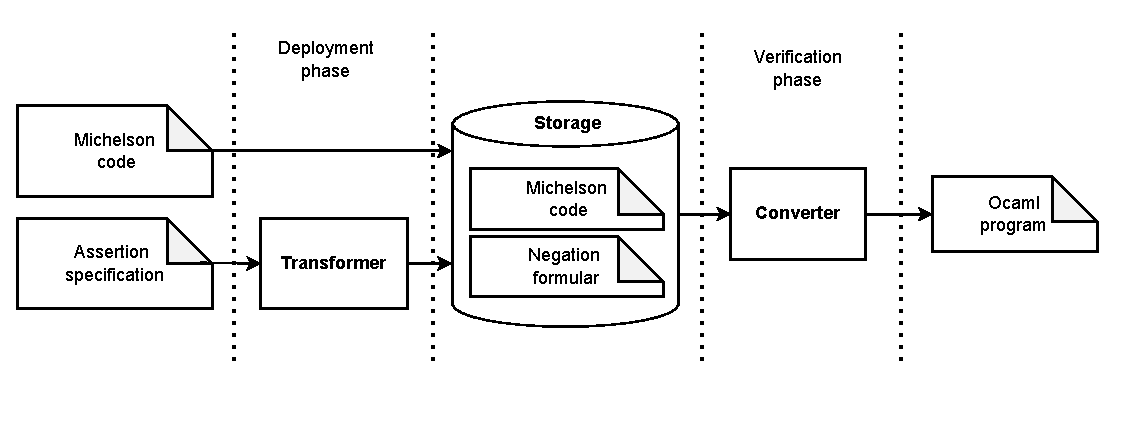
\includegraphics[scale=0.65]{assertion-tezos}
\caption{The architecture}
\label{fig.architect}
\end{figure}
\todo{disscus and implement}
\section{Experiment and Cost Analysis}
\label{sec:cost-analysis}
\end{document}


